\begin{figure}[h]
	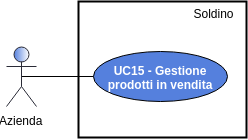
\includegraphics[width=5cm]{res/images/UC15-Generale.png}
	\centering
	\caption{UC15 - Gestione prodotti in vendita}
\end{figure}
\subsubsection{UC15 - Gestione prodotti in vendita}
\begin{itemize}
	\item \textbf{Attori Primari}: azienda;
	\item \textbf{Descrizione}: le aziende hanno la possibilità di gestire i propri beni in vendita sulla piattaforma;
	\item \textbf{Scenario principale}: l'azienda accede alla pagina per la gestione dei beni/servizi venduti e può:
	\begin{itemize}
		\item inserire un nuovo prodotto da vendere [UC15.1];
		\item visualizzare i propri prodotti attualmente in vendita [UC15.2];
		\item modificare un prodotto già presente nella piattaforma [UC15.3];
		\item rimuovere un prodotto presente [UC15.4].
	\end{itemize}
	\item \textbf{Precondizione}: il sistema ha identificato l'utente come azienda, l'azienda si trova nella pagina per la gestione dei propri beni/servizi;
	\item \textbf{Postcondizione}: il sistema fornisce all'azienda le operazioni che possono essere svolte sui propri beni/servizi.	
\end{itemize}
\begin{figure}[h]
	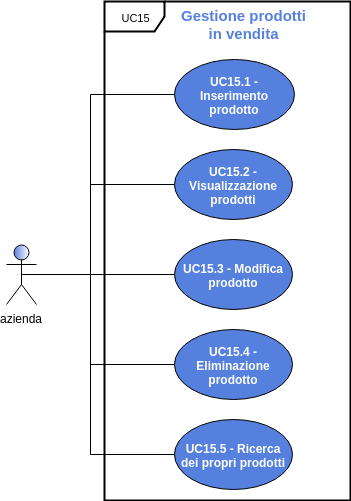
\includegraphics[width=7cm]{res/images/UC15.png}
	\centering
	\caption{UC15.1 - Gestione prodotti in vendita, sottocasi}
\end{figure}
\subsubsection{UC15.1 - Inserimento prodotto}
\begin{figure}[h]
	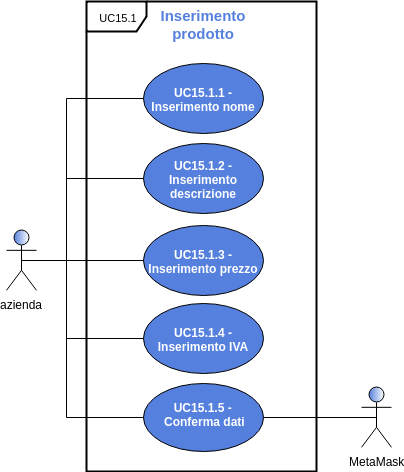
\includegraphics[width=8cm]{res/images/UC15-1.png}
	\centering
	\caption{UC15.1 - Inserimento prodotto, sottocasi}
\end{figure}
\begin{itemize}
	\item \textbf{Attori Primari}: azienda;
	\item \textbf{Attori Secondari}: MetaMask\glo;
	\item \textbf{Descrizione}: le aziende possono inserire dei nuovi prodotti nella piattaforma;
	\item \textbf{Scenario principale}: l'azienda accede alla pagina per inserire un nuovo prodotto e deve:
	\begin{enumerate}[label=\alph*.]
			\item inserire il nome del bene/servizio [UC15.1.1];
		\item inserire la descrizione del bene/servizio [U15.1.2];
		\item inserire il prezzo netto unitario del bene/servizio [UC15.1.3];
		\item inserire l'IVA del bene/servizio [UC15.1.4];
		\item confermare i dati inseriti [UC15.1.5].
	\end{enumerate}
	
	\item \textbf{Precondizione}: il sistema ha identificato l'utente come azienda, l'azienda si trova nella pagina di gestione dei beni/servizi;
	\item \textbf{Postcondizione}: l'azienda ha inserito correttamente i dati relativi al nuovo prodotto ed è riuscita ad inserire il nuovo prodotto sulla piattaforma.	
\end{itemize}
\subsubsection{UC15.1.1 - Inserimento nome}
\begin{itemize}
	\item \textbf{Attori Primari}: azienda;
	\item \textbf{Descrizione}: al fine di portare a termine il processo di inserimento di un nuovo prodotto l'azienda deve inserire il nome del prodotto, campo ritenuto obbligatorio;
	\item \textbf{Scenario principale}: l'azienda compila il campo relativo al nome del nuovo prodotto da inserire;
	\item \textbf{Precondizione}: il sistema ha reso disponibile il form per l'inserimento di un nuovo prodotto, in particolare è presente il campo per l'inserimento del nome;
	\item \textbf{Postcondizione}: l'azienda ha compilato il campo relativo al nome del nuovo prodotto da inserire.
\end{itemize}
\subsubsection{U15.1.2 - Inserimento descrizione}
\begin{itemize}
	\item \textbf{Attori Primari}: azienda;
	\item \textbf{Descrizione}: al fine di portare a termine il processo di inserimento di un nuovo prodotto l'azienda deve inserire la descrizione del prodotto, campo ritenuto obbligatorio;
	\item \textbf{Scenario principale}: l'azienda compila il campo relativo alla descrizione del nuovo prodotto da inserire;
	\item \textbf{Precondizione}: il sistema ha reso disponibile il form per l'inserimento di un nuovo prodotto, in particolare è presente il campo per l'inserimento della descrizione;
	\item \textbf{Postcondizione}: l'azienda ha compilato il campo relativo alla descrizione del nuovo prodotto da inserire.
\end{itemize}
\subsubsection{UC15.1.3 - Inserimento prezzo netto}
\begin{itemize}
	\item \textbf{Attori Primari}: azienda;
	\item \textbf{Descrizione}: al fine di portare a termine il processo di inserimento di un nuovo prodotto l'azienda deve inserire il prezzo netto unitario del prodotto, campo ritenuto obbligatorio;
	\item \textbf{Scenario principale}: l'azienda compila il campo relativo al prezzo del nuovo prodotto da inserire;
	\item \textbf{Precondizione}: il sistema ha reso disponibile il form per l'inserimento di un nuovo prodotto, in particolare è presente il campo per l'inserimento del prezzo;
	\item \textbf{Postcondizione}: l'azienda ha compilato il campo relativo al prezzo del nuovo prodotto da inserire.
\end{itemize}
\subsubsection{UC15.1.4 - Inserimento IVA}
\begin{itemize}
	\item \textbf{Attori Primari}: azienda;
	\item \textbf{Descrizione}: al fine di portare a termine il processo di inserimento di un nuovo prodotto l'azienda deve inserire l'aliquota\glosp IVA che intende applicare al prodotto;
	\item \textbf{Scenario principale}: l'utente compila il campo relativo all'aliquota\glosp IVA del nuovo prodotto da inserire;
	\item \textbf{Precondizione}: il sistema ha reso disponibile il form per l'inserimento di un nuovo prodotto, in particolare è presente il campo per l'inserimento dell'aliquota\glosp IVA;
	\item \textbf{Postcondizione}: l'azienda ha compilato il campo relativo all'aliquota\glosp IVA del nuovo prodotto da inserire.
\end{itemize}
\subsubsection{UC15.1.5 - Conferma dati}
\begin{itemize}
	\item \textbf{Attori Primari}: azienda;
	\item \textbf{Attori Primari}: MetaMask\glo;
	\item \textbf{Descrizione}: al fine di portare a termine il processo di inserimento di un prodotto, l'azienda deve confermare i dati inseriti tramite l'approvazione della transazione, che verrà eseguita attraverso il plug-in MetaMask\glo;
	\item \textbf{Scenario principale}: l'azienda preme il pulsante di conferma dei dati inseriti e valida la transazione con MetaMask\glo;
	\item \textbf{Precondizione}: il sistema ha reso disponibile il form per l'inserimento dei dati riguardanti il nuovo prodotto, l'azienda ha compilato tutti i campi ed ha premuto il pulsante per la conferma;
	\item \textbf{Postcondizione}: il nuovo prodotto è stato inserito nella piattaforma e l'azienda visualizza un messaggio di conferma della riuscita dell'operazione.
\end{itemize}

\subsubsection{UC15.2 - Visualizzazione prodotto}
\begin{itemize}
	\item \textbf{Attori Primari}: azienda;
	\item \textbf{Descrizione}: le aziende possono visualizzare i loro prodotti inseriti nella piattaforma. Per ogni prodotto l'azienda può visualizzarne:
	\begin{itemize}
		\item il nome;
		\item la descrizione;
		\item il prezzo netto unitario;
		\item la percentuale IVA imposta.
	\end{itemize}
	\item \textbf{Scenario principale}: l'azienda accede alla pagina per visualizzare i loro prodotti in vendita;	

	\item \textbf{Precondizione}: il sistema ha identificato l'utente come azienda, questa ha acceduto alla pagina del proprio account dedicata alla gestione dei prodotti da essa messi in vendita;
	\item \textbf{Postcondizione}: l'azienda ha ottenuto la lista dei propri prodotti assieme alle operazioni eseguibili su di essi.	
\end{itemize}

\subsubsection{UC15.3 - Modifica prodotto}
\begin{figure}[H]
	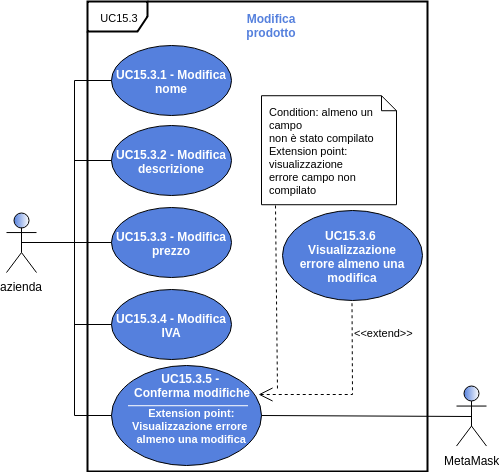
\includegraphics[width=10cm]{res/images/UC15-3.png}
	\centering
	\caption{UC15.3 - Modifica prodotto, sottocasi}
\end{figure}
\begin{itemize}
	\item \textbf{Attori Primari}: azienda;
	\item \textbf{Attori Secondari}: MetaMask\glo;
	\item \textbf{Descrizione}: le aziende possono modificare i loro prodotti inseriti nella piattaforma. In particolare potrà:
	 \begin{itemize}
		\item modificarne il nome [UC15.3.1];
		\item modificarne la descrizione [UC15.3.2];
		\item modificarne il prezzo [UC15.3.3];
		\item modificarne l'IVA [UC15.3.4].
		
	\end{itemize}
	Per ognuno dei campi verrà messo a disposizione il valore attuale ed un campo per inserire il nuovo valore;

	\item \textbf{Scenario principale}: l'azienda accede alla modifica di un prodotto attraverso l'apposito pulsante mostrato assieme alle informazioni riguardanti l'oggetto stesso[UC15.2]. Dunque: 
	\begin{enumerate}[label=\alph*.]
		\item modificare uno o più campi come sopra descritto;
		\item confermare le modifiche [UC15.3.5];
	\end{enumerate}
	Infine dovrà confermare l'operazione attraverso l'utilizzo di MetaMask\glo{};
	
	\item \textbf{Precondizione}: il sistema ha identificato l'utente come azienda e l'azienda si trova sulla pagina di modifica delle informazioni di un particolare prodotto, dopo aver cliccato sull'apposito pulsante di modifica del prodotto desiderato;
	\item \textbf{Postcondizione}: l'azienda ha modificato le caratteristiche del prodotto. Il sistema visualizza un messaggio per avvisare l'utente del successo dell'operazione.
\end{itemize}

\subsubsection{UC15.3.1 - Modifica nome}
\begin{itemize}
	\item \textbf{Attori Primari}: azienda;
	\item \textbf{Descrizione}: l'azienda inserisce nell'apposito campo il nuovo nome del prodotto;
	\item \textbf{Scenario principale}: l'utente visualizza il vecchio nome con affianco un campo dati per inserire il nuovo nome ed inserisce il nuovo valore;
	\item \textbf{Precondizione}: il sistema ha reso disponibile il form per la modifica dei dati relativi ad un prodotto messo in vendita dall'azienda;
	\item \textbf{Postcondizione}: l'azienda ha inserito il nuovo nome nel campo dedicato del form.
\end{itemize}

\subsubsection{UC15.3.2 - Modifica descrizione}
\begin{itemize}
	\item \textbf{Attori Primari}: azienda;
	\item \textbf{Descrizione}: l'azienda inserisce nell'apposito campo la nuova descrizione del prodotto;
	\item \textbf{Scenario principale}: l'utente visualizza la vecchia descrizione con affianco un campo dati per inserire la nuova descrizione, ed inserisce il nuovo valore;
	\item \textbf{Precondizione}: il sistema ha reso disponibile il form per la modifica dei dati relativi ad un prodotto messo in vendita dall'azienda;
	\item \textbf{Postcondizione}: l'azienda ha inserito la nuova descrizione nel campo dedicato del form.
\end{itemize}

\subsubsection{UC15.3.3 - Modifica prezzo}
\begin{itemize}
	\item \textbf{Attori Primari}: azienda;
	\item \textbf{Descrizione}: l'azienda inserisce nell'apposito campo il nuovo prezzo del prodotto;
	\item \textbf{Scenario principale}: l'utente visualizza il vecchio prezzo con affianco un campo dati per inserire il nuovo prezzo ed inserisce il nuovo valore;
	\item \textbf{Precondizione}: il sistema ha reso disponibile il form per la modifica dei dati relativi ad un prodotto messo in vendita dall'azienda;
	\item \textbf{Postcondizione}: l'azienda ha inserito il nuovo prezzo nel campo dedicato del form.
\end{itemize}

\subsubsection{UC15.3.4 - Modifica aliquota IVA}
\begin{itemize}
	\item \textbf{Attori Primari}: azienda;
	\item \textbf{Descrizione}: l'azienda inserisce nell'apposito campo la 
	nuova aliquota IVA imposta al prodotto;
	\item \textbf{Scenario principale}: l'utente visualizza la vecchia aliquota 
	IVA con affianco un campo dati per inserire il nuovo valore, e compila 
	tale campo;
	\item \textbf{Precondizione}: il sistema ha reso disponibile il form per la modifica dei dati relativi ad un prodotto messo in vendita dall'azienda;
	\item \textbf{Postcondizione}: l'azienda ha inserito la nuova aliquota IVA imposta nel campo dedicato del form.
\end{itemize}

\subsubsection{UC15.3.5 - Conferma modifiche}
\begin{itemize}
	\item \textbf{Attori Primari}: azienda;
	\item \textbf{Attori Primari}: MetaMask\glo;
	\item \textbf{Descrizione}: al fine di portare a termine il processo di modifica dei dati di un bene/servizio, l'utente deve confermare i dati inseriti tramite l'approvazione della transazione, che verrà eseguita attraverso il plug-in MetaMask\glo;
	\item \textbf{Scenario principale}: l'utente preme il pulsante di conferma dei dati inseriti e valida l'operazione con MetaMask\glo;
	\item \textbf{Estensioni}:
	\begin{itemize}
		\item \textbf{UC15.3.6}: l'utente tenta di confermare i dati senza aver compilato almeno uno dei campi.
	\end{itemize}
	\item \textbf{Precondizione}: il sistema ha reso disponibile il form per la modifica dei dati riguardanti un prodotto. L'utente ha compilato almeno un campo ed ha premuto il pulsante per la conferma;
	\item \textbf{Postcondizione}: il prodotto è stato aggiornato con i nuovi dati. Il sistema visualizza un messaggio per avvisare l'utente del fatto che l'operazione è stata eseguita con successo.
\end{itemize}


\subsubsection{UC15.3.6 - Visualizzazione errore almeno una modifica}
\begin{itemize}
	\item \textbf{Attori Primari}: azienda;
	\item \textbf{Descrizione}:
	l'utente visualizza un messaggio di errore relativo al fatto nessuno dei campi per la modifica è stato compilato, e che quindi non è possibile attuare alcuna modifica;
	\item \textbf{Scenario principale}: l'utente tenta di confermare ed inviare le modifiche ai dati senza aver compilato almeno uno dei campi del form;
	\item \textbf{Precondizione}: il sistema permette all'utente di compilare il form per le modifiche. L'utente ha premuto il pulsante di conferma senza aver modificato almeno uno dei campi; 
	\item \textbf{Postcondizione}:
	viene visualizzato un messaggio d'errore per informare l'utente del fatto che, per effettuare una modifica, almeno uno dei dati presenti deve essere stato modificato. È dunque necessario compilare almeno uno dei campi del form.
\end{itemize}

\subsubsection{UC15.4 - Eliminazione prodotto}
\begin{itemize}
	\item \textbf{Attori Primari}: azienda;
	\item \textbf{Attori Primari}: MetaMask\glo;
	\item \textbf{Descrizione}:
	l'azienda elimina uno dei propri beni/servizi presenti sulla piattaforma;
	\item \textbf{Scenario principale}: l'utente clicca sul pulsante di eliminazione prodotto, mostrato assieme alle informazioni riguardanti l'oggetto stesso [UC15.2]. Dunque dovrà confermare l'operazione attraverso l'utilizzo di MetaMask\glo;
	\item \textbf{Inclusione}:
	\begin{itemize}
		\item \textbf{UC15.2}: per poter eliminare i prodotti l'azienda deve prima individuarli nella lista dei propri prodotti.
	\end{itemize}
	\item \textbf{Precondizione}: il sistema ha identificato l'utente come azienda, l'azienda è acceduta alla pagina relativa alla visualizzazione e gestione dei prodotti da essa venduti nella piattaforma;
	\item \textbf{Postcondizione}: l'azienda ha eliminato il prodotto. Il sistema ha visualizzato un messaggio che conferma il successo dell'operazione.
\end{itemize}

\subsubsection{UC15.5 - Ricerca dei propri prodotti}
\begin{itemize}
	\item \textbf{Attori Primari}: azienda;
	\item \textbf{Descrizione}:
	l'azienda può effettuare la ricerca di un proprio prodotto tra quelli che ha inserito nella piattaforma;
	\item \textbf{Scenario principale}: l'azienda accede alla pagina in cui sono presenti i loro prodotti in vendita e inserisce nella casella di ricerca il nome del prodotto che vuole cercare;
	\item \textbf{Precondizione}: il sistema ha identificato l'utente come azienda, questa ha acceduto alla pagina del proprio account dedicata alla gestione dei prodotti da essa messi in vendita e ha digitato nella casella di ricerca il nome del prodotto interessato;
	\item \textbf{Postcondizione}:
	 l'azienda ha ottenuto il prodotto o la lista dei prodotti che corrispondono al nome digitato, assieme alle operazioni eseguibili su di esso/i.
\end{itemize}


